\documentclass[logo,reportComp]{thesis}
\usepackage[cpp,pseudo]{mypackage}

\title{操作系统原理实验报告}
\subtitle{实验九:线程模型}
\school{数据科学与计算机学院}
\author{陈鸿峥}
\classname{17大数据与人工智能}
\stunum{17341015}
\headercontext{操作系统原理实验报告}
% \authorremark{本实验报告用\LaTeX撰写,创建时间:\builddate\today}

\begin{document}

\maketitle

\section{实验目的}
\begin{itemize}
	\item 理解并实现线程模型
	\item 能够编写运行一些简单的多线程程序
\end{itemize}

\section{实验要求}
% 实验目的和实验要求由老师提供实验项目文档中获取
\begin{enumerate}
\item 在内核中实现线程,并在C库中封装相关的系统调用。
\item 利用多线程技术,在进程中创建两个子线程,分别显示5个“Hello”和“world!”。
\end{enumerate}

\section{实验环境}
% 包括:硬件或虚拟机配置方法、软件工具与作用、方案的思想、相关原理、程序流程、算法和数据结构、程序关键模块,结合代码与程序中的位置进行解释。不得抄袭,否则按作弊处理。
% 实验方案包括相关基础原理、实验工具和环境、程序流程和算法思想、数据结构与程序模块功能说明,代码文档组成说明等
具体环境选择原因已在实验一报告中说明。
\begin{itemize}
	\item Windows 10系统 + Ubuntu 18.04(LTS)子系统
	\item gcc 7.3.0 + nasm 2.13.02 + GNU ld (Binutils) 2.3.0
	\item GNU Make 4.1
	\item Oracle VM VirtualBox 6.0.6
	\item Bochs 2.6.9
	\item Sublime Text 3 + Visual Studio Code 1.33.1
\end{itemize}

虚拟机配置:内存4M,1.44M虚拟软盘引导,1.44M虚拟硬盘。

\section{实验方案}
% 包括:主要工具安装使用过程及截图结果、程序过程中的操作步骤、测试数据、输入及输出说明、遇到的问题及解决情况、关键功能或操作的截图结果。不得抄袭,否则按作弊处理。
{\textbf{\textcolor{red}{本次实验继续沿用实验六保护模式的操作系统。用户程序都以ELF文件格式读入,并且在用户态(ring 3)下执行。}}}

本次实验借鉴了Linux操作系统对线程进程的管理,采用\textbf{进程和线程统一管理的方法},即进程与线程都可以看作是一个\verb'task',在调度、执行、管理上面都不进行区分。

这一方面大大减少了冗余的代码量,另一方面也使进程和线程的管理更加简单。
为了避免进程fork时开销过大的问题,Linux采用了当写时才复制(Copy On Write, COW)机制,即\verb'fork'时不将进程所对应的全部进程空间进行复制,而是采用以下方案:
\begin{itemize}
	\item 在GDT表项中将父进程和子进程的数据段都置为只读
	\item 当实际运行中遇到父进程或子进程对数据段进行修改时,触发异常,硬件中断,进入中断处理程序
	\item 这时才将进程空间进行拷贝
\end{itemize}
这将很大程度上降低进程\verb'fork'的开销,也使进程线程的复制能够统一化管理。

由于Linux任务管理的这种特性,我们也将线程称为轻量级进程(lightweight process)。
因此,我们不需要对原有的\verb'task.h'头文件进行修改,而只需添加一些线程设施。

\subsection{线程创建}
线程创建与进程的\verb'fork'类似,但要注意下面的函数原型,多了三个参数传递,这是与进程\verb'fork'非常不同的地方。
\begin{lstlisting}
int do_thread_create(int* tid, uintptr_t func, void* args)
\end{lstlisting}
其中,
\begin{itemize}
	\item \verb'tid':返回线程ID
	\item \verb'func':多线程函数调用入口
	\item \verb'args':函数参数
\end{itemize}

具体的步骤如下
\begin{itemize}
	\item 用\verb'proc_alloc'分配一个新的任务
	\item 将当前进程主线程控制块的内容拷贝至子线程中
	\item 修改栈段指针\verb'ebp'和\verb'user_esp',并拷贝主线程栈中所有内容
	\item 设置子线程的状态
	\item 设置函数入口\verb'eip=func',同时将函数参数\verb'args'和返回地址\verb'user_pthread_return'堆栈,注意这里\verb'user_pthread_return'必须是用户态(ring 3)程序可以执行的,否则会报GPF错。
	实现方法即利用用户态中断\verb'int 0x81',重返内核。
	\item 最后设置\verb'tid'的返回值
\end{itemize}

完整函数如下所示。
\begin{lstlisting}
int do_thread_create(int* tid, uintptr_t func, void* args)
{
	disable();

	process* child;

	// find empty entry
	if ((child = proc_alloc()) == 0) {
		enable();
		return -1; // fail to create child process
	}

	// copy PCB, which has been saved by interrupt
	child->regImg.eip = curr_proc->regImg.eip;
	child->regImg.cs = curr_proc->regImg.cs;
	child->regImg.eflags = curr_proc->regImg.eflags;

	child->regImg.eax = curr_proc->regImg.eax;
	child->regImg.ecx = curr_proc->regImg.ecx;
	child->regImg.edx = curr_proc->regImg.edx;
	child->regImg.ebx = curr_proc->regImg.ebx;

	child->regImg.esp = curr_proc->regImg.esp;
	child->regImg.ebp = curr_proc->regImg.ebp + (child->pid * 0x100); // use different stack!
	child->regImg.esi = curr_proc->regImg.esi;
	child->regImg.edi = curr_proc->regImg.edi;

	child->regImg.ds = curr_proc->regImg.ds;
	child->regImg.es = curr_proc->regImg.es;
	child->regImg.fs = curr_proc->regImg.fs;
	child->regImg.gs = curr_proc->regImg.gs;

	child->regImg.ss = curr_proc->regImg.ss;
	child->regImg.user_esp = curr_proc->regImg.user_esp + (child->pid * 0x100);

	// copy stack
	memcpy((void*)(child->regImg.user_esp),
		(void*)(curr_proc->regImg.user_esp),
		(curr_proc->regImg.ebp - curr_proc->regImg.user_esp)*2); // each entry 32-bit

	// set state
	child->regImg.eax = 0;
	child->parent = curr_proc;
	child->status = PROC_READY;
	reset_time(child);

	// set function entrance
	child->regImg.eip = func;
	uintptr_t* stack = (uintptr_t*) child->regImg.user_esp;
	stack--;
	*stack = (uintptr_t) args; // pass arguments
	stack--;
	*stack = (uintptr_t) user_pthread_return; // return address
	child->regImg.user_esp = (uintptr_t) stack;

	// set return values
	*tid = child->pid;

	return 0;
}
\end{lstlisting}

\subsection{线程等待}
此函数主要用在主线程,用来等待子线程完成。
实现方法即将主线程设置为\verb'PROC_WAITING',然后进入任务调度阶段,继续执行子线程。
\begin{lstlisting}
void do_thread_join(int tid, void** ret)
{
	disable();
	curr_proc->status = PROC_WAITING;
	schedule_proc();
	enable();
}
\end{lstlisting}

\subsection{线程退出}
将当前线程状态设为终止,然后将其父进程唤醒。
从这里也可以看出,一个\verb'exit'函数对应着一个\verb'join'函数,故有多少个线程,为了同步就应该有多少个\verb'join'。
这与Linux的\verb'pthread'库实现方式是一样的。
\begin{lstlisting}
void do_thread_exit()
{
	disable();
	curr_proc->status = PROC_TERMINATED;
	if (curr_proc->parent != NULL)
		wakeup(curr_proc->parent->pid);
	enable();
}
\end{lstlisting}

为方便用户函数调用,也提供了用户态的退出函数\verb'user_pthread_return'
\begin{lstlisting}
void user_pthread_return() {
	asm volatile (
		"int 0x81\n\t"
		:
		:"a"(3)
		);
}
\end{lstlisting}

此函数需要添加在每个线程函数的最后,即堆栈返回地址,否则将无法回到主线程继续执行。

\subsection{系统调用}
为了不让单一系统调用太过复杂,本实验的\verb'pthread'采用\verb'int 0x81'号中断调用。
通过下列函数对IDT进行设置,确保用户态程序可以调用。
\begin{lstlisting}
setvect_user (0x81, (unsigned long) sys_pthread_handler);
\end{lstlisting}

其中\verb'sys_pthread_handler'是一个汇编入口,将寄存器信息都保存后,进入\verb'sys_pthread_handler_main'中断处理程序。
先将\verb'ebx,ecx,edx'寄存器的内容取出,其中含有用户传递的参数;然后依次进入线程管理程序进行处理。
注意这里都是以\verb'uintptr_t'的32位地址格式传递,进入函数后才进行类型转换。
\begin{lstlisting}
extern void sys_pthread_handler ();
int sys_pthread_handler_main (int no) {
	uintptr_t arg1, arg2, arg3;
	asm volatile("":"=b"(arg1):);
	asm volatile("":"=c"(arg2):);
	asm volatile("":"=d"(arg3):);
	if (no == 0) {
		return do_thread_create((int*) arg1, arg2, (void*) arg3);
	} else if (no == 1) {
		do_thread_join((int) arg1, (void**) arg2);
	} else if (no == 2) {
		return do_thread_self();
	} else if (no == 3) {
		do_thread_exit();
	}
	return 0;
}
\end{lstlisting}

对这些函数进行封装,得到\verb'pthread.h'头文件,API如下,基本与Linux的POSIX线程库相同:
\begin{itemize}
	\item \verb'int pthread_create(int* tid, uintptr_t func, void* args)':创建线程
	\item \verb'void pthread_join(int tid, void** ret)':线程等待
	\item \verb'int pthread_self()':获取线程ID
	\item \verb'void pthread_exit()':线程退出
\end{itemize}

\section{实验结果}
\subsection{多线程Hello world测试}
用户程序\verb'hello_world_thread.c'代码如下。
\begin{lstlisting}
#include "stdio.h"
#include "pthread.h"

int m = 5;

void hello(void* args){
	char* str = (char*) args;
	for(int i = 0; i < m; i++)
		printf("%s\n", str);
}

void main() {
	int tid1, tid2;
	pthread_create(&tid1,(uintptr_t)hello,"Hello");
	pthread_create(&tid2,(uintptr_t)hello,"world!");
	pthread_join(tid1,NULL);
	pthread_join(tid2,NULL);
	return;
}
\end{lstlisting}

实验结果如图\ref{fig:hello_world}所示。
\begin{figure}[H]
\centering
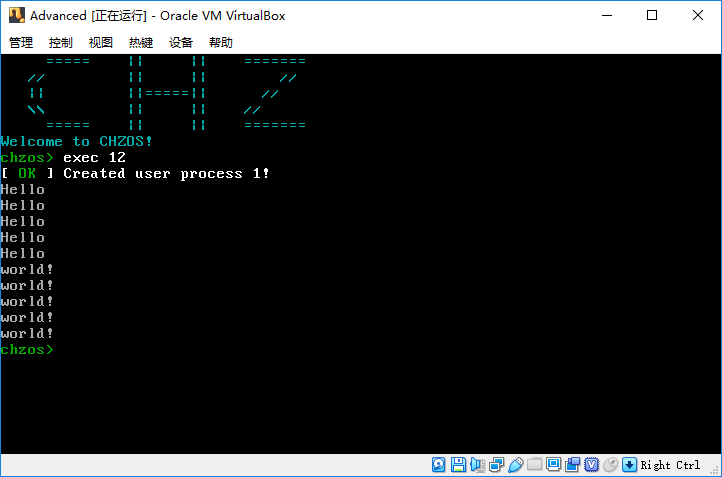
\includegraphics[width=0.8\linewidth]{fig/hello_world.PNG}
\caption{多线程Hello world($m=5$)}
\label{fig:hello_world}
\end{figure}
由于线程执行的速度非常快,故即使设置轮转时间片大小为1,线程也都执行完了。

为真正展现多线程执行的效果,我将$m$值调大,使其输出多个\verb'Hello'和多个\verb'world!',以便观察多个线程的并发关系。

从图\ref{fig:hello_world_2}中可以看出,两个线程确实是交替执行的,\verb'Hello'和\verb'world!'相互穿插,甚至有在输出换行期间中断造成线程调度的。
从此可以看出多线程程序执行的不确定性,这确实是符合预期的。
\begin{figure}[H]
\centering
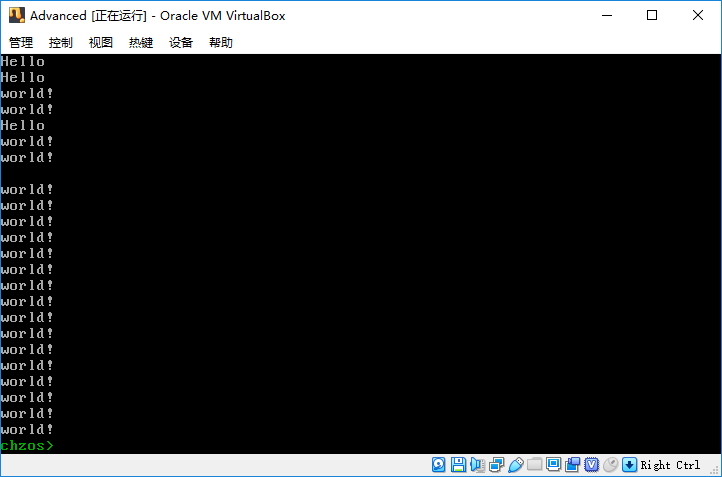
\includegraphics[width=0.8\linewidth]{fig/hello_world_2.PNG}
\caption{多线程Hello world($m=100$)}
\label{fig:hello_world_2}
\end{figure}

\subsection{多线程矩阵乘法测试}
除了前面简单的Hello world测试,我也编写了稍微复杂一点的程序。
如下所示是一个多线程的矩阵乘法,采用数据并行的方法进行划分计算。
\begin{lstlisting}
#include "stdio.h"
#include "pthread.h"

// maximum size of matrix 
#define MAX 6

// maximum number of threads 
#define MAX_THREAD 3

int matA[MAX][MAX];
int matB[MAX][MAX];
int matC[MAX][MAX];

void multiply(void* arg)
{
	int tid = pthread_self();
	printf("This is thread:%d Arg:%d\n", tid, (int)arg);

	int core = (int) arg;
	// Each thread computes 1/n of the matrix multiplication 
	for (int i = core * MAX / MAX_THREAD; i < (core + 1) * MAX / MAX_THREAD; i++) 
		for (int j = 0; j < MAX; j++) 
			for (int k = 0; k < MAX; k++){
				// printf("%d ", i);
				matC[i][j] += matA[i][k] * matB[k][j];
			}
}

int main() 
{ 
	// Generating values in matA and matB 
	for (int i = 0; i < MAX; i++) { 
		for (int j = 0; j < MAX; j++) { 
			matA[i][j] = i + j; 
			matB[i][j] = i * j;
			matC[i][j] = 0;
		} 
	} 

	// Displaying matA 
	printf("Matrix A\n"); 
	for (int i = 0; i < MAX; i++) { 
		for (int j = 0; j < MAX; j++) 
			printf("%d ", matA[i][j]); 
		printf("\n");
	} 

	// Displaying matB 
	printf("Matrix B\n");
	for (int i = 0; i < MAX; i++) { 
		for (int j = 0; j < MAX; j++) 
			printf("%d ", matB[i][j]); 
		printf("\n");
	} 

	// declaring four threads 
	pthread_t threads[MAX_THREAD]; 

	// Creating four threads, each evaluating its own part 
	for (int i = 0; i < MAX_THREAD; i++)
		pthread_create(&threads[i], (pthread_addr)multiply, (void*)(i));

	// joining and waiting for all threads to complete 
	for (int i = 0; i < MAX_THREAD-1; i++) 
		pthread_join(threads[i], NULL);
	pthread_join(threads[MAX_THREAD-1], NULL);

	// Displaying the result matrix 
	printf("Multiplication of A and B\n");
	for (int i = 0; i < MAX; i++) { 
		for (int j = 0; j < MAX; j++) 
			printf("%d ", matC[i][j]); 
		printf("\n");
	} 
	return 0; 
}
\end{lstlisting}

从图\ref{fig:matmul}中可以看出,即使面向复杂的多线程程序,我的操作系统依然可以正常运行,且结果正确。
\begin{figure}[H]
\centering
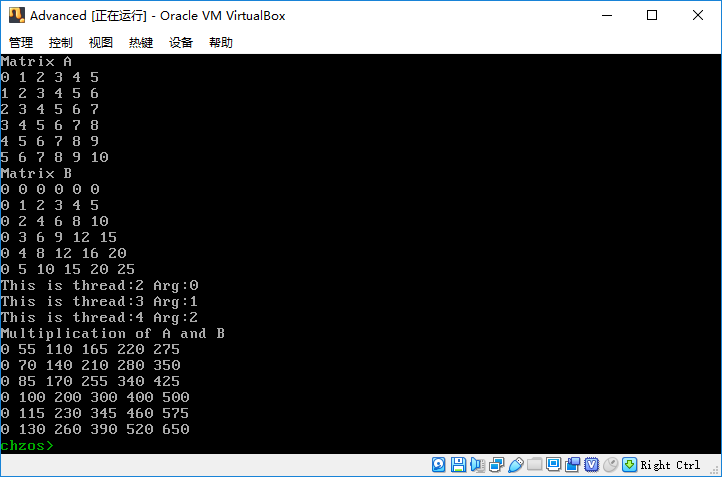
\includegraphics[width=0.8\linewidth]{fig/matmul.PNG}
\caption{多线程矩阵乘法}
\label{fig:matmul}
\end{figure}

\section{实验总结}
% 每人必需写一段,文字不少于500字,可以写心得体会、问题讨论与思考、新的设想、感言总结或提出建议等等。不得抄袭,否则按作弊处理。
本次实验主要在前期线程模型方面纠结了较长时间,不知道线程控制块应该怎么设置。
后来了解到Linux的进程线程管理模型,瞬间醍醐灌顶,不得不说Linux的实现真的非常妙。

传统教材中都将进程和线程分开来处理,而Linux却将这两者看成是等价的,既能实现更细粒度的管理,又能结合COW等机制将进程管理的开销降到最低。
因此,基于这个理论,我操作系统的线程实现就非常迅速了。
不需要对原有的进程模型进行修改,而只需添加对多线程的支持。

以前常想操作系统已经发展了几十年了,Windows也已到最后一代Win 10,这样操作系统还有什么可以做的呢。
这其实是不对的,操作系统是一个充满活力的学科,课本上的理论都是上个世纪的东西,随着操作系统的不断发展,很多实现也与当初的理论大相径庭,但是却能实现性能、稳定性、安全性等的大幅提升。
本次实验实现了类Linux的进程模型,相较课本上的进程线程模型更为紧凑而优美,这也算是我迈向现代操作系统的第一步吧。

由并行分布式课程会用POSIX编写一些多线程程序,再到操作系统能自己实现\verb'pthread'库,看着多线程程序在我眼前飞舞,我能感受到从上到下一脉打通的快感,也真真切切感受到了现代计算机的无比魅力。

\section{参考资料}
\begin{enumerate}
	\item OS Development Series, \url{http://www.brokenthorn.com/Resources/OSDevIndex.html}
	\item Roll your own toy UNIX-clone OS, \url{http://www.jamesmolloy.co.uk/tutorial_html/}
	\item The little book about OS development, \url{http://littleosbook.github.io/}
	\item Writing a Simple Operating System from Scratch, \url{http://www.cs.bham.ac.uk/~exr/lectures/opsys/10_11/lectures/os-dev.pdf}
	\item Intel$^{\textregistered}$ 64 and IA-32 Architectures Software Developer's Manual
	\item UCore OS Lab, \url{https://github.com/chyyuu/ucore_os_lab}
	\item CMU CS 15-410, Operating System Design and Implementation, \url{https://www.cs.cmu.edu/~410/}
	\item 李忠,王晓波,余洁,《x86汇编语言-从实模式到保护模式》,电子工业出版社,2013
\end{enumerate}

\appendix
\appendixconfig
\section{程序清单}
\subsection{内核核心代码}
\begin{center}
\begin{tabular}{|c|l|l|}\hline
\textbf{序号} & \textbf{文件} & \textbf{描述} \\\hline
1 & \verb'bootloader.asm' & 主引导程序\\\hline
2 & \verb'kernel_entry.asm' & 内核汇编入口程序\\\hline
3 & \verb'kernel.c' & 内核C入口程序\\\hline
4 & \verb'Makefile' & 自动编译指令文件\\\hline
5 & \verb'bootflpy.img' & 引导程序/内核软盘\\\hline
6 & \verb'mydisk.hdd' & 虚拟硬盘\\\hline
7 & \verb'bochsrc.bxrc' & Bochs配置文件\\\hline
\end{tabular}
\end{center}

\subsection{内核头文件}
\begin{center}
\begin{tabular}{|c|l|l|}\hline
\textbf{序号} & \textbf{文件} & \textbf{描述} \\\hline
1 & \verb'disk_load.inc' & BIOS读取磁盘\\\hline
2 & \verb'show.inc' & 常用汇编字符显示\\\hline
3 & \verb'gdt.inc' & 汇编全局描述符表\\\hline
4 & \verb'gdt.h' & C全局描述符表\\\hline
5 & \verb'idt.h' & 中断描述符表\\\hline
6 & \verb'hal.h' & 硬件抽象层\\\hline
6.1 & \verb'pic.h' & 可编程中断控制器\\\hline
6.2 & \verb'pit.h' & 可编程区间计时器\\\hline
6.3 & \verb'keyboard.h' & 键盘处理\\\hline
6.4 & \verb'tss.h' & 任务状态段\\\hline
6.5 & \verb'ide.h' & 硬盘读取\\\hline
7 & \verb'io.h' & I/O编程\\\hline
8 & \verb'exception.h' & 异常处理\\\hline
9 & \verb'syscall.h' & 系统调用\\\hline
10 & \verb'task.h' & 多进程设施\\\hline
11 & \verb'user.h' & 用户程序处理\\\hline
12 & \verb'terminal.h' & Shell\\\hline
13 & \verb'scancode.h' & 扫描码\\\hline
14 & \verb'stdio.h' & 标准输入输出\\\hline
15 & \verb'string.h' & 字符串处理\\\hline
16 & \verb'elf.h' & ELF文件处理\\\hline
17 & \verb'api.h' & 进程管理API\\\hline
18 & \verb'semaphore.h' & 信号量机制\\\hline
19 & \verb'systhread.h' & 线程模型\\\hline
20 & \verb'pthread.h' & 线程管理API\\\hline
\end{tabular}
\end{center}

\subsection{用户程序}
用户程序都放置在\verb'usr'文件夹中。
\begin{center}
\begin{tabular}{|c|l|l|}\hline
\textbf{序号} & \textbf{文件} & \textbf{描述} \\\hline
1-4 & \verb'prgX.asm' & 飞翔字符用户程序\\\hline
5 & \verb'box.asm' & 画框用户程序\\\hline
6 & \verb'sys_test.asm' & 系统中断测试\\\hline
7 & \verb'fork_test.c' & 进程分支测试\\\hline
8 & \verb'fork2.c' & 进程多分支测试\\\hline
9 & \verb'bank.c' & 银行存取款测试\\\hline
10 & \verb'fruit.c' & 父子祝福水果测试\\\hline
11 & \verb'prod_cons.c' & 消费者生产者模型测试\\\hline
12 & \verb'hello_world_thread.c' & 多线程Hello\_world测试\\\hline
13 & \verb'matmul.c' & 多线程矩阵乘法测试\\\hline
\end{tabular}
\end{center}

\section{系统调用清单}
\label{sec:syscall}
\begin{center}
\begin{tabular}{|c|c|}\hline
\verb'int 0x80'\textbf{功能号} & \textbf{功能}\\\hline
0 & 输出OS Logo\\\hline
1 & 睡眠100ms\\\hline
10 & \verb'fork'\\\hline
11 & \verb'wait'\\\hline
12 & \verb'exit'\\\hline
13 & \verb'get_pid'\\\hline
20 & \verb'get_sem'\\\hline
21 & \verb'sem_wait'\\\hline
22 & \verb'sem_signal'\\\hline
23 & \verb'free_sem'\\\hline
100 & 返回内核Shell\\\hline
\end{tabular}
\end{center}

\begin{center}
\begin{tabular}{|c|c|}\hline
\verb'int 0x81'\textbf{功能号} & \textbf{功能}\\\hline
0 & \verb'pthread_create'\\\hline
1 & \verb'pthread_join'\\\hline
2 & \verb'pthread_self'\\\hline
3 & \verb'pthread_exit'\\\hline
\end{tabular}
\end{center}

\end{document}

% 实验提交内容
% 实验报告:电子版(Word2003的DOC格式或PDF格式)
% 原程序文件及可执行代码程序文件
% 测试输入数据文件和输出数据文件
% 虚拟机软盘映像文件

% 基础实验项目5个和扩展实验7个
% 实验项目,迟交影响成绩评价!
% 工具与环境可由选择,开发新型工具或优化一套开发环境都可加分!
% 一系列基础实验项目必须连续完成,当前项目只能在前一个项目的基础上进行,体现出前后的进化关系,否则要被约谈,证明没有抄袭行为!
% 一个项目可提交多个改进的版本,实现新功能和个性化特征都有利于提高相应项目的成绩。
% 实验项目提交内容用winrar工具整体压缩打包,统一格式命名为:
%	<学号>+<姓名>+<实验项目号>+<版本号>.rar
%	姓名(学号)实验NvX.zip
%	实验报告、项目文件夹、映像文件
%	ftp://172.18.216.232 sysuac 下周六23:59

% 免考
% 条件:实验1~6全部评价AAAAB+B+或相当
% 最终成绩可能范围:75分以上